\chapter{How to Use GERT}

It would be silly for this thesis to present a software toolkit and then
neglect to show how to use it.

\section{API Inspiration}
GERT's API is based on Arduino's because of its remarkable simplicity. In order to
get started with GERT on a Freescale iMX6 SOC, the programmer must only implement three functions: \textit{user\_init},
\textit{user\_loop} and \textit{irq}. \textit{user\_init} should contain code that is run only once
on startup, \textit{user\_loop} should contain the main event loop of the embedded program, and
\textit{irq} is the IRQ handler.

\section{Writing Interrupt Handlers}

Since interrupts can happen even while the world is stopped, the programmer must make sure that \textit{irq} never executes
a blocking Go function or allocates memory on the Go heap with \textit{make()}. These constraints are
easily manageable by breaking the program interrupt logic into two pieces: a monitoring
goroutine which watches a boolean flag, and the interrupt service routine which sets the flag.
For example, a NIC (Network Interface Controller) driver may use interrupts to determine when a new frame should be retrieved
from the NIC. Rather than reading the new frame in the interrupt routine, the NIC driver
can set a flag in the interrupt routine so that a seperate thread inside the NIC driver can retrieve
the new frame. This seperate thread is just an ordinary goroutine with no constraints on the type
of code it can execute.

\section{Building a GERT Program}

\begin{figure}[h]
\begin{center}
  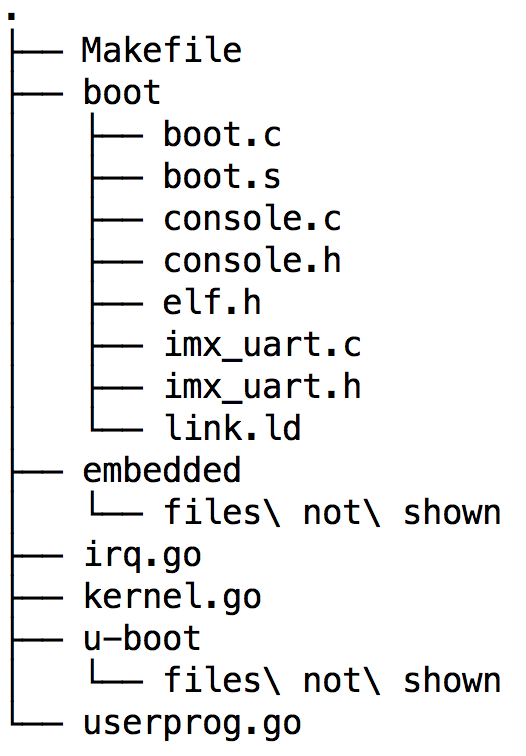
\includegraphics[scale=0.5]{dirtree}
\end{center}
  \caption{GERT Program Directory Layout} \label{fig:dtree}
\end{figure}

GERT needs a bootloader
and entry point to start on bare metal. The directory structure of a GERT
program is shown in fig. \ref{fig:dtree}. The boot directory contains the GERT
bootloader as well as linker script for it. Userprog.go and irq.go contain
the user-implemented functions as well as the user-implemented irq handler.
Kernel.go does three mundane things: it defines a new entry point for the Go runtime
(which just sets a flag so the runtime knows it is booting on bare metal),
it also finishes booting additional CPU's, and it configures the ARM Generic Interrupt Controller \cite{gic} for normal operation. The makefile
is responsible for stitching the bootloader and GERT program together into an
SD card image for u-boot. It uses \textit{go build} to build the GERT program
with the modified Go runtime and then inserts the GERT program as a binary blob
into the bootloader's data section. The makefile also includes a target which writes
u-boot and the final GERT binary to an SD card.

\section{Design Considerations}
Every SOC has a different memory map and peripherals, so GERT must be adjusted
accordingly. In order to change the link address of GERT, pass "-T <link address>"
as a link flag into \textit{go build}. The link address of the bootloader also needs
to be changed too inside \textit{link.ld}. It is good practice to link the bootloader in an
area of RAM that can be reclaimed once GERT enables paging.

\section{Writing Drivers}
GERT imposes no driver model on the programmer. All drivers in
GERT should be written as normal Go code in the best style for
the intended application. GERT exposes no safe methods for reading
or writing device memory so any MMIO peripherals in the SOC must be
carefully programmed using the \textit{unsafe} package. Most MMIO
peripherals arrange their registers contiguously in memory so they
can be represented with a Go struct, which requires only one unsafe cast
for initial assignment.

GERT currently comes with an example driver
library in the form of a package called \textit{embedded}. The \textit{embedded} package is not intrinsic to GERT's
functionality, nor was it optimized for performance in any way. The \textit{embedded} package
just aims to provide a template for how drivers can be written in the Go language.
It only functions for the Freescale i.MX6 and includes drivers for the UART, SPI, PWM, GIC, USDHC, GPIO, and GPT peripherals.
The package also includes a generic implementation of the FAT32 file system, which is
layered on top of a \textit{read} and \textit{write} function that the programmer can define.


